\documentclass[a4paper,titlepage,12pt]{article}
\usepackage[utf8]{inputenc}
\usepackage{todonotes}
\usepackage{url}
\usepackage{listings}
\usepackage{color}
\usepackage{subcaption}
\begin{document}
 
\newcommand{\horrule}[1]{\rule{\linewidth}{#1}}     % Horizontal rule

\title{
        %\vspace{-1in}  
        \usefont{OT1}{bch}{b}{n}
        \normalfont \normalsize \textsc{KU Leuven} \\ [25pt]
        \normalfont \normalsize \textsc{Computer Vision} 
        \horrule{2pt} \\[0.5cm]
        \huge Final Project: Incisor Segmentation \\
        \horrule{2pt} \\[0.5cm]
}
\author{
        \normalfont            
        Joran Van de Woestijne (r0378602)\\
        Tim Van Den Broecke (r0296620)
}
\date{August 2017}
 
\maketitle

\newpage
\tableofcontents
\thispagestyle{empty}
\newpage
\setcounter{page}{1}

\section{Introduction}
\todo[inline]{TODO: Joran}

\section{Shape Model}
\todo[inline]{TODO: Tim}

\subsection{Shape alignment}

\subsection{PCA analysis}

\section{Radiograph pre-processing}

Dental radiographs are inherently noisy and contain too much information when just focusing on locating the upper and lower incisors.
For instance, all the teeth (not just the incisors), the jaw and the nose are present in the radiographs.
To reduce these radiographs to a more suitable size for our application, we crop them based on domain knowledge so that only the smaller region around the four incisors remains.

After the size reduction, the radiographs still need to be de-noised so that it's easier for our algorithm to detect the edges.
We achieve this by using the technique proposed in \textit{Noise Removal and Contrast Enhancement for X-Ray Images} by Huang et al \cite{JBEMI1893}.
The algorithm proposed by Huang et al is visualised in Figure \ref{preprocessalgo}. This technique first starts off by applying an adaptive median filter to reduce the impulsive (salt-and-pepper) noise, after which a bilateral filter is used to suppress the Gaussian noise while also preserving the edges of the image.
After the noise suppression step, the radiograph is sharpened by a mathematical morphology, here a top hat and bottom hat transform.
The top hat transform enhances the brighter regions of the radiograph, whereas the bottom hat enhances the darker regions.
Finally, the contrast of the radiograph is enhanced by applying a contrast limited adaptive histogram equalization (CLAHE).
To detect the edges of the dental radiograph, a Sobel operator is used, detecting the gradients in the x and y direction.
The results of applying the different pre-processing steps on a dental radiograph can be observed in Figure \ref{preprocess}. 


\begin{figure}
\centering
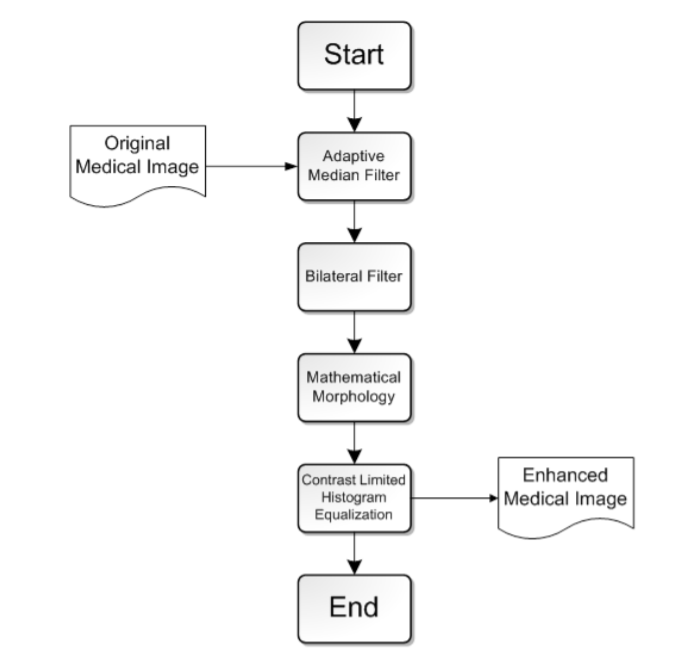
\includegraphics[width=0.7\linewidth]{preprocess/algorithm.png}
  \caption{
		The algorithm proposed by Huang et al \cite{JBEMI1893} for denoising dental radiographs. The algorithm has four steps, with a top hat transform and a bottom hat transform representing the mathematical morphology step. } \label{preprocessalgo}
\end{figure}

\begin{figure}
  \centering
	\begin{minipage}[b]{0.32\linewidth}
		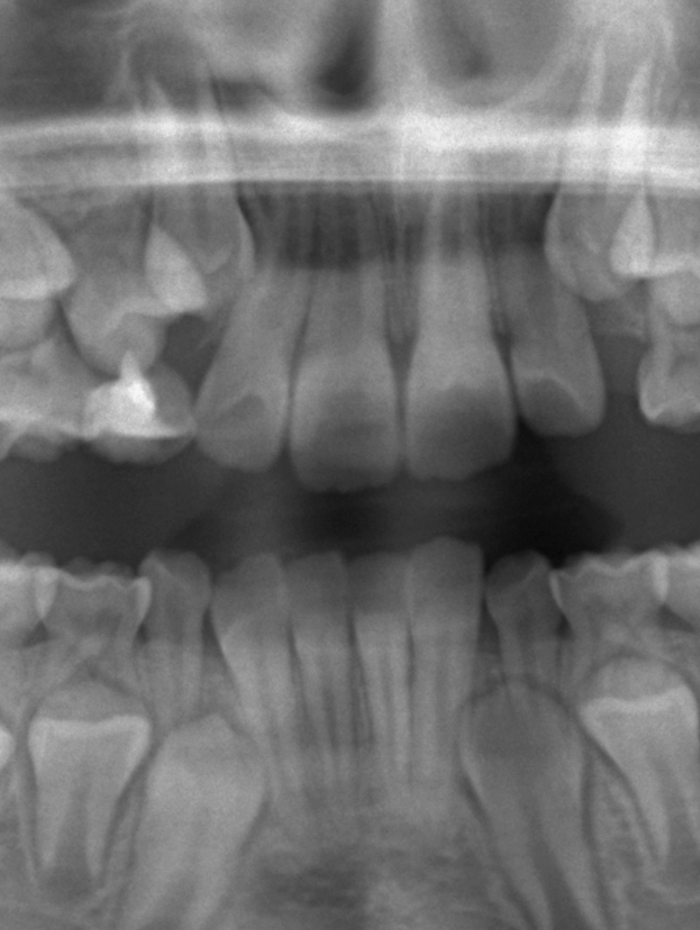
\includegraphics[width=\linewidth]{preprocess/original.png}
		\subcaption{Cropped}
	\end{minipage}
	\begin{minipage}[b]{0.32\linewidth}
		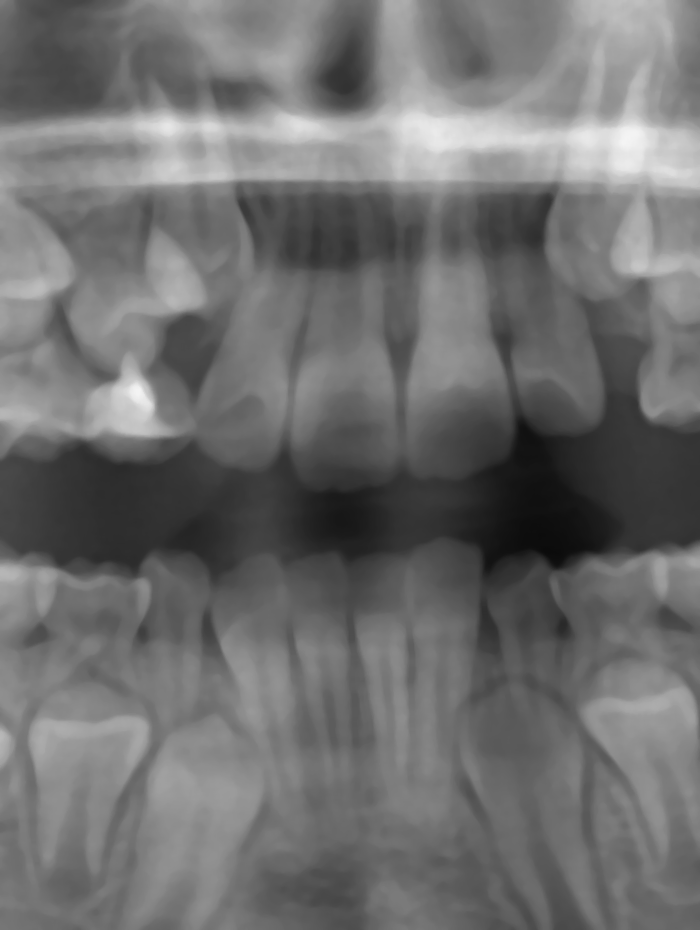
\includegraphics[width=\linewidth]{preprocess/median.png}
		\subcaption{Median filter}
	\end{minipage}
	\begin{minipage}[b]{0.32\linewidth}
		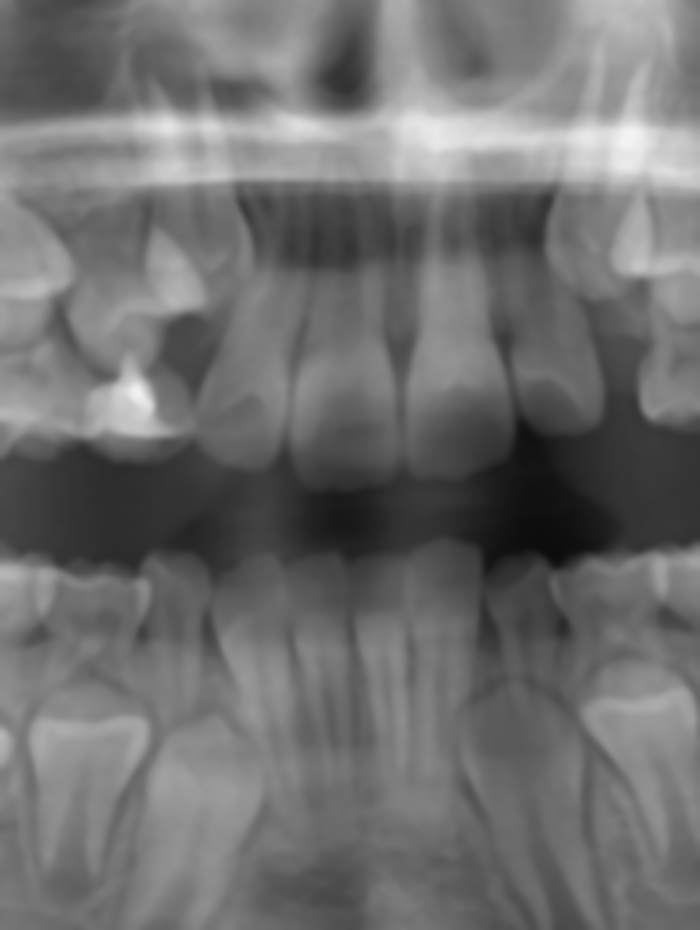
\includegraphics[width=\linewidth]{preprocess/bilateral.png}
		\subcaption{Bilateral Filter}
	\end{minipage}
	\begin{minipage}[b]{0.32\linewidth}
		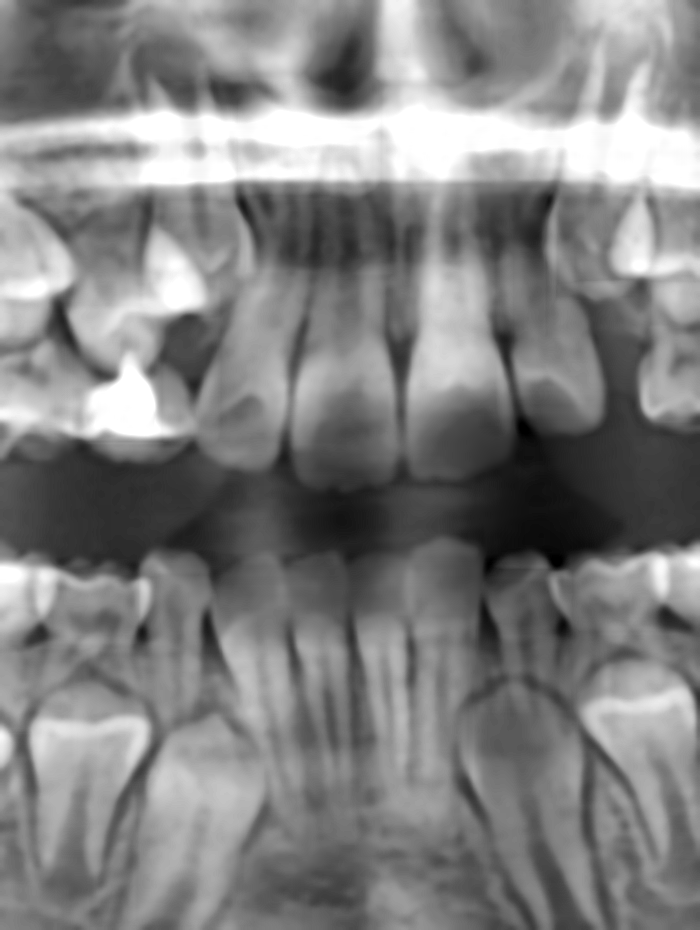
\includegraphics[width=\linewidth]{preprocess/hats.png}
		\subcaption{Top and Bottom hat}
	\end{minipage}
	\begin{minipage}[b]{0.32\linewidth}
		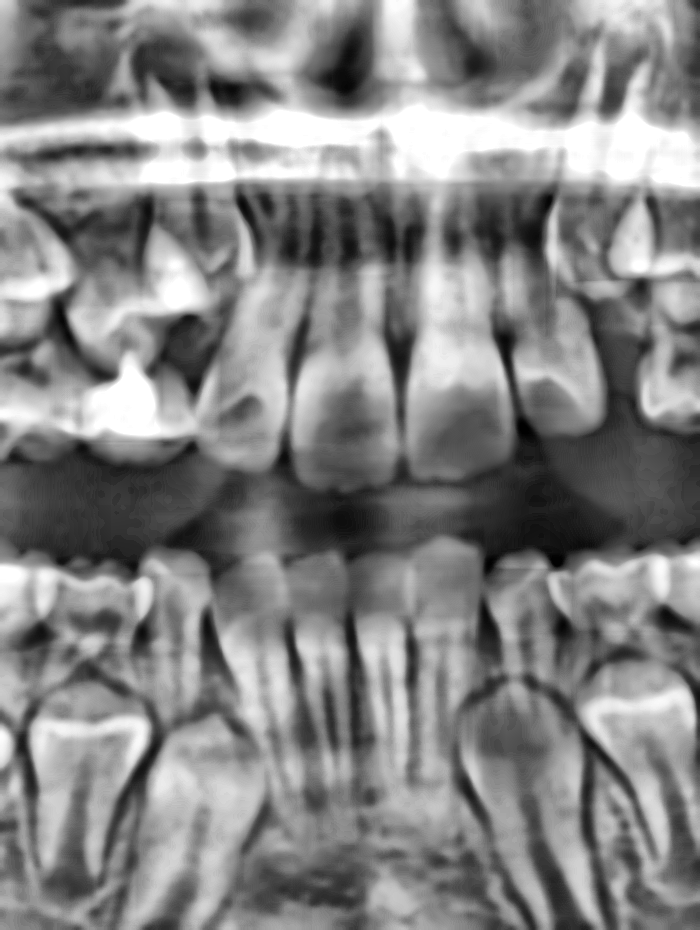
\includegraphics[width=\linewidth]{preprocess/clahe.png}
		\subcaption{CLAHE}
	\end{minipage}
	\begin{minipage}[b]{0.32\linewidth}
		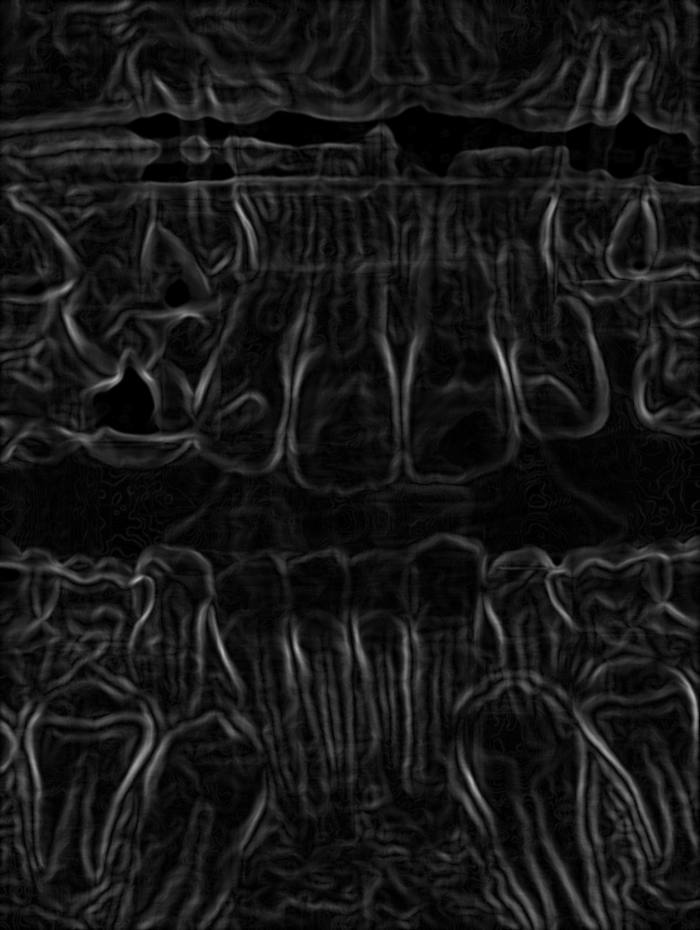
\includegraphics[width=\linewidth]{preprocess/gradients.png}
		\subcaption{Edges (Sobel)}
	\end{minipage}
  \caption{
		The results of the different pre-processing steps visualised when applied on dental radiograph 3.
		(a) shows the original image after cropping, (b) shows (a) after applying the adaptive median filter, (c) adds the bilateral filter onto the result of (b), (d) performs the mathematical morphology (top hat and bottom hat) on (c), and (e) finally applies CLAHE. A Sobel operator is used to detect the edges, which is visualised in (f).} \label{preprocess}
\end{figure}


\section{Fitting model to image}
To fit our model to an image, we have to find the model instance $x =T_{(tx,ty,s,\theta)}(\bar{x} + Pb)$ that most accurately aligns with the incisors in the image.
This translates to finding the pose parameters $T_{(tx,ty,s,\theta)}$ and the shape parameters $b$.
This is achieved in two steps: In the first step, an initial estimate for the pose parameters is obtained, which is discussed in Section \ref{subsec:initial} . The second step finally fits the model to the image by applying the Active Shape Model algorithm, which is discussed in Section \ref{subsec:ASM}

\subsection{Initial pose estimate}
\label{subsec:initial}

To determine an initial estimate for the pose parameters $T_{(tx,ty,s,\theta)}$, we need to find an estimate for the horizontal offset $tx$, the vertical offset $ty$, the scale $s$ and the rotation $\theta$.

\paragraph{Scale and rotation}

To find an initial estimate for the scale and rotation, we use domain knowledge. A good scale was empirically determined, and the rotation is chosen so that the teeth are positioned vertically.

\paragraph{Vertical offset}

To find the vertical offset $ty$, we utilise the jaw separation of the radiograph.
This is accomplished by first finding the jaw separation that separates the upper incisors from the lower incisors, which corresponds to the pixel row that has the lowest total intensity value. After having found this separation, a small region above and below this separation is considered to locate the upper and lower offset where the teeth actually start. This is achieved by looking at the pixel row with the highest gradient in this region, which is caused by the transition from the black background to the white teeth.
This technique was able to correctly determine the vertical offset for 12/14 images for the upper landmarks and 13/14 images for the lower landmarks.
The result of locating the vertical offset can be observed in Figure \ref{init}(a).

\paragraph{Horizontal offset}

To find the horizontal offset $tx$, we use a hough line transform to detect the boundary between the middle incisors.
For the upper incisors, a small region above the vertical offset is considered, near the center of the image.
A hough line transform is applied on this small region to detect the boundaries between the different teeth.
The line closest to the middle of this region then represents the boundary between the middle incisors, which we use as the horizontal offset.
The results of this can be observed in Figure \ref{init}(b).
The method works analogously for the lower incisors, but now a small region below the vertical offset is considered. 
This is visualised in Figure \ref{init}(c).
This method was able to correctly determine the horizontal offset for 13/14 images for the upper landmarks and 13/14 images for the lower landmarks.


\begin{figure}
  \centering
	\begin{minipage}[b]{0.32\linewidth}
		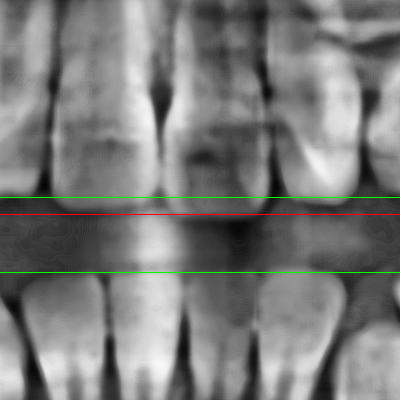
\includegraphics[width=\linewidth]{init/sep.png}
		\subcaption{Jaw separation}
	\end{minipage}
	\begin{minipage}[b]{0.32\linewidth}
		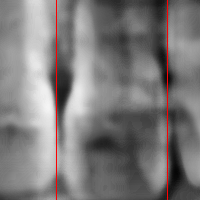
\includegraphics[width=\linewidth]{init/up.png}
		\subcaption{Upper hough lines}
	\end{minipage}
	\begin{minipage}[b]{0.32\linewidth}
		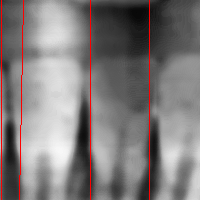
\includegraphics[width=\linewidth]{init/down.png}
		\subcaption{Lower hough lines}
	\end{minipage}
	\begin{minipage}[b]{0.32\linewidth}
		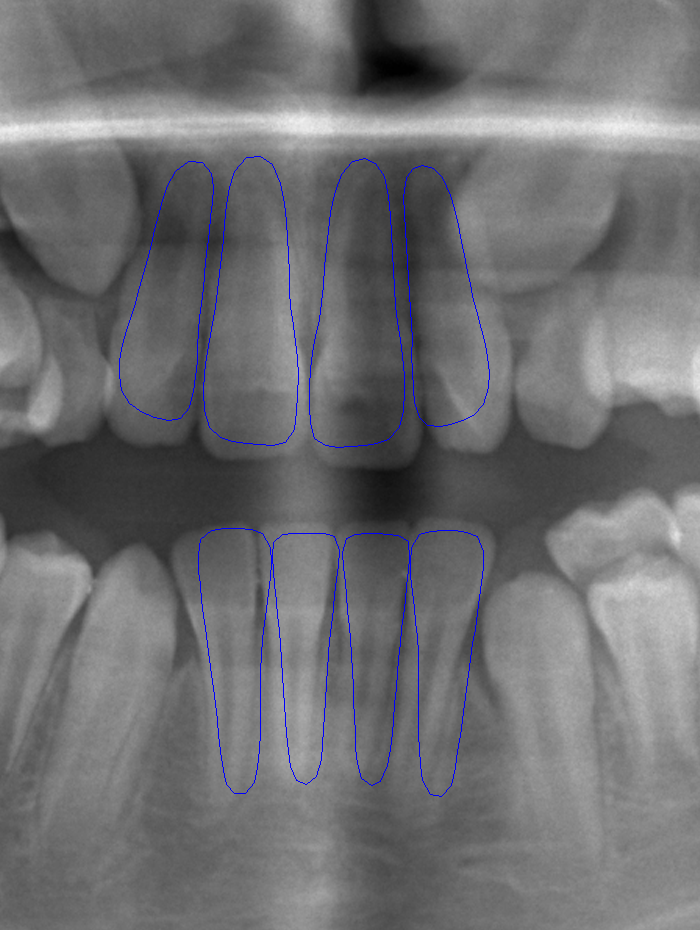
\includegraphics[width=\linewidth]{init/initial.png}
		\subcaption{Result for image 11}
	\end{minipage}
	\begin{minipage}[b]{0.32\linewidth}
		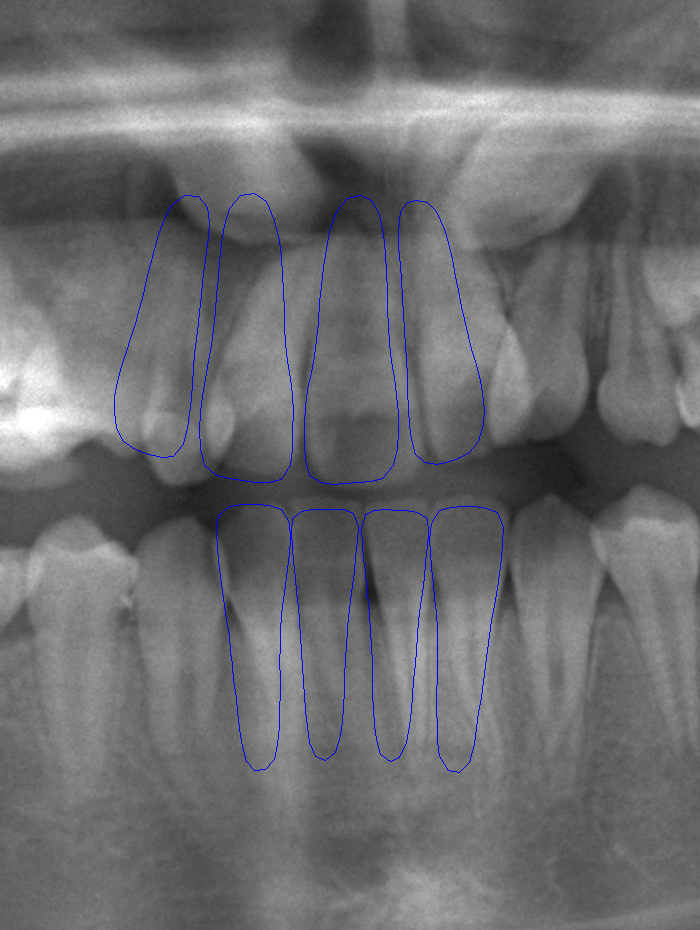
\includegraphics[width=\linewidth]{init/initial6.png}
		\subcaption{Result for image 5}
	\end{minipage}
  \caption{
		The process of getting the initial pose estimate. (a) shows the jaw separation lines for radiograph 11, where the red line shows the row of pixels with the lowest intensity and the green lines show the resulting upper and lower jaw separations.
		(b) and (c) show the hough lines for the upper and lower incisors respectively for radiograph 11.
		(d) shows the resulting initial estimate for radiograph 11, which is a really good fit, and (e) shows the initial estimate for radiograph 5.
		The estimate for radiograph 5 is a lot worse due to the off-centered position of the upper incisors.} \label{init}
\end{figure}

\subsection{The ASM algorithm}
\label{subsec:ASM}

\section{Evaluation}

\todo[inline]{TODO: Tim}

\section{Conclusion}

\todo[inline]{TODO: Tim, if even necessary after evaluation?}

\bibliography{references}
\bibliographystyle{plain}

\end{document}
